\documentclass[journal]{IEEEtran}
\ifCLASSINFOpdf
\else
\fi

\usepackage{todonotes}
\usepackage{datetime}

\newdateformat{curMonth}{\monthname[\THEMONTH],~\THEYEAR}

%\hyphenation{op-tical net-works semi-conduc-tor}
\begin{document}
\title{An analysis of the Delta Correlating Prediction Table prefetcher}

\author{Ingebrigt~Bartholsen,~Christian~Chavez,~Solveig~Fure~and~Andreas~Hammar,~\IEEEmembership{Students,~NTNU}}


%\thanks{J. Doe and J. Doe are with Anonymous University.}
%\thanks{Manuscript received April 19, 2005; revised December 27, 2012.}}

% The paper headers
\markboth{An~analysis~of~the~Delta~Correlating~Prediction~Table~prefetcher,~TDT4260,~April~2014\hfill\curMonth}{}

% make the title area
\maketitle

\begin{abstract}
Abstract goes here... 
\end{abstract}


% Note that keywords are not normally used for peerreview papers.
\begin{IEEEkeywords}
DCPT, Prefetcher, NTNU, TDT4260, 2014, Computer Architecture.
\end{IEEEkeywords}
\IEEEpeerreviewmaketitle

\curMonth
\hfill \today
\section{Introduction}

\IEEEPARstart{T}{he} ``memory wall'' is becoming an increasing challenge for the
computers of tomorrow. This ``memory wall'' is when the on-chip computing speeds
exceed the on-chip memory capacities, creating the situation where computing
circuitry has to lie idle waiting for instructions/data to arrive from off-chip
locations and be put into the on-chip cache. The cache is the fastest, most
expensive, and most sparingly used memory resource in a computer, more often
than not residing as closely on-chip as possible to the \emph{central processing
unit} (CPU). One method for reducing this gap is called \emph{prefetching}.

The idea behind prefecthing is to have a predictive module moving
instructions/data from the slower off-chip memory (like main memory) to the much
faster cache \emph{before} it is needed. Hence, when the processor then requires
the instruction/data, it is already in the cache and can be made use of within
an amount of on-chip clock cycles, not having to wait for the slower off-chip
clock cycles dominated by the time it takes for one or more chips to communicate
(like on a bus).

The purpose of this report is to develop and evaluate a prefetcher using the M5
simulator, with a prefetcher utilizing maximum 8KiB. We implement a DCPT
prefetcher, as this design proves to be very effective. The prefetcher is
implemented according to the algorithm presented in ``Storage Efficient Hardware
Prefetching using Delta Correlation Prediction Tables'' by Grannaes, Jahre, and
Natvig~\cite{dcpt}. The storage limitation makes it important to examine how the
8 KiB can be used most efficiently. \todo[inline]{Possible physical implementation will be
discussed(?).}

\todo[inline]{About the introduction:
- Introduces the larger research area that the paper is
a part of\\
- Introduces the problem at hand\\
- Explains the scheme\\}


\section{Background}

In this section, we go over the algorithmic details of the two prefetchers we
have chosen to implement, detailing how we intend our implemented prefetchers
to work.

\subsection{TS Prefetching Algorithm}

The simplest prefetcher is the sequential prefetcher, which fetches the next
block of data~\cite{seq}. The TS prefetcher is a slight improvement over the
sequential prefetcher. As with sequential prefetching, the spatial locality of
data is exploited.

Additionally, a tagging system is used to mark the cache blocks that have been
prefetched. This system is used to recognize when a prefetched cache block is
accessed by the application, which implies that there has been a successful
prefetch. Subsequent blocks are prefetched into the cache when there has been a
cache miss, or when a previously prefetched cache entry has been
accessed~\cite{grannaes}.

The TS prefetcher can be configured by adjusting two parameters; the
\emph{distance} is how many blocks ahead of the currently accessed block the
prefetcher will fetch, and the \emph{degree} is how many consequtive blocks it
will fetch starting at this location in memory.

\subsection{Delta Correlating Prefetching Table Algorithm}

The DCPT prefetcher uses a more advanced algorithm. It is an instruction-based
prefetcher using a table indexed by the address of the instruction which tried
to access memory.

Each entry in this table utilizes a ring buffer for keeping track of the deltas,
and therefore organizing the memory this table needs effectively is an important
aspect. In the original implementation~\cite{dcpt} which we based our
implementation on, only 4KiB of storage are used.

Each entry contains a ring buffer of the most recent deltas between successive
addresses accessed by this instruction.

When an access happens, the prefetcher examines the two most recent deltas and
searches the ring buffer for patterns beginning with these two deltas. If there
are multiple matches, we choose the longest matching sequence of deltas.

The prefetcher then adds the found delta pattern to the current address to
obtain the predicted stream of future accesses. It discards addresses which
are already in the cache, or ones that are already being prefetched. It then
issues prefetch commands for the remaining addresses.


\section{Prefetcher Description}

\todo[inline]{The prefetcher description goes here. Another section title maybe?
\\
- Explain your scheme in detail\\
- Choose an informative title\\
- Trick: Add an informative figure that helps explain
your scheme\\
- If your scheme is complex, an informative example
may be in order\\}

\subsection{Delta Correlating Prediction Table}

\subsection{Tagged Sequential}

The tagged sequential prefetcher is a slight improvement over the sequential
prefetcher. Preceeding (etterfølgende?) blocks are prefetched to the cache when
there has been a cache miss, or when a previously prefetched cache entry has
been accessed. \todo{Vet ikke om dette med distance stemmer helt..) Our tagged
sequential prefetcher was implemented with (..........)}The prefetching degree
determines how many blocks should be prefetched at a time, and the distance
specifies how many blocks away from the currently accessed block the prefetches
should be done.

\subsubsection{Hardware requirements}

With the given implementation, a tagged sequential prefetcher simply requires
one bit per cache word in order to store the associated tag. With an L2 cache
size of 1 MB and 64 bit word size, there are 128 different words in the cache,
meaning 128 bits of storage is required for the tagged prefetcher.


\section{Methodology}

Hardware components must usually be designed within an area budget, and in order
to simulate realistic conditions, the implemented prefetchers are limited to a
maximum of 8KiB memory~\cite{guidelines}. The simulations are performed by the
M5 simulator available on the Kongull HPC cluster at NTNU.

Both prefetchers are implemented as described, and then simulated with different
configurations in order to seach for patterns and then optimize each prefetcher
to the benchmarks used.

\subsection{The M5 Simulator}
The M5 simulator used in our testing only utilizes a subset of its rich
feature set~\cite{user_doc}, due to the time limitation of this report. The simulator runs several of the SPEC CPU2000 benchmarks available on the
pfJudge course website~\cite{guidelines}. The benchmarks considered in this
report are; ``\emph{ammp}'', ``\emph{applu}'', ``\emph{apsi}'',
``\emph{art110}'', ``\emph{art470}'', ``\emph{bzip2\_graphic}'',
``\emph{bzip2\_program}'', ``\emph{bzip2\_source}'', ``\emph{galgel}'',
``\emph{swim}'', ``\emph{twolf}'', and ``\emph{wupwise}''.

It is important that the prefetcher performance is evaluated with a variety of
benchmarks representing typical applications. The mentioned benchmarks are
widely used and recognized. We also believe that the results give a proper
foundation for performance evaluation\footnote{For more information about the
benchmarks, please see \emph{www.spec.org}.}.

The prefetcher simulation scores reported in \ref{sec:res} are averages of the
the speed-up with the abovementioned benchmarks. The speed-up is a measure on how
much faster M5 runs (number of instructions per clock cycle) with one of our
prefetchers compared to no prefetching at all.

\todo[inline]{Needs more details? I don't know -C}

\subsection{TS Tests}

When testing the TS prefetcher, we vary both the \emph{distance} and the
\emph{degree} parameters it uses. The distances tested are in the range of 2 to
20, and the degree from 1 to 4.

The intention of testing the TS prefetcher, is to have a benchmark to compare
the DCPT prefetcher against. Hence, we use the averaged scores given by the
pfJudge website~\cite[Sec.~2.5]{guidelines} of this course when comparing
results.

\subsection{DCPT Tests}

When testing the DCPT prefetcher we vary the \emph{table size}, \emph{delta
size} and \emph{delta ring buffer size}. Initially, these parameters are set to

the optimal values found by
\todo[inline]{Fix the name of below reference. M. Jahre is not good enough}
M. Jahre\cite{dcpt}; table size 98, delta size 19 and ring buffer size 12.
Although these values are obtained with different benchmarks and with a maximum
4KiB prefetcher size, it is a reasonable starting point. The impact of each
parameter is then studied by keeping two of them constant while varying the
third.

Since our implementation has 8KiB available, double of
\todo[inline]{Same as previous/other reference.}
M. Jahres \cite{dcpt}
has, we can exploit this by having larger tables, delta-sizes, and ring buffer
size. Our analysis will reveal wich parameter combinations that works best.

After this analysis we simulate with the optimal values of each parameter.

\todo[inline]{Explain your experimental setup\\
- Which simulator did you use?\\
- How have you extended the simulator?\\
- Which parameters did you use for your simulations? (aim: reproducibility)\\
- Which benchmarks did you use?\\
- Why did you chose these benchmarks?\\
$=>$ Important: should be realistic}


\section{Results}
\label{sec:res}

\subsection{TS Results}

\begin{figure}[h!]
	\begin{centering}
		% GNUPLOT: LaTeX picture with Postscript
\begingroup
  \makeatletter
  \providecommand\color[2][]{%
    \GenericError{(gnuplot) \space\space\space\@spaces}{%
      Package color not loaded in conjunction with
      terminal option `colourtext'%
    }{See the gnuplot documentation for explanation.%
    }{Either use 'blacktext' in gnuplot or load the package
      color.sty in LaTeX.}%
    \renewcommand\color[2][]{}%
  }%
  \providecommand\includegraphics[2][]{%
    \GenericError{(gnuplot) \space\space\space\@spaces}{%
      Package graphicx or graphics not loaded%
    }{See the gnuplot documentation for explanation.%
    }{The gnuplot epslatex terminal needs graphicx.sty or graphics.sty.}%
    \renewcommand\includegraphics[2][]{}%
  }%
  \providecommand\rotatebox[2]{#2}%
  \@ifundefined{ifGPcolor}{%
    \newif\ifGPcolor
    \GPcolorfalse
  }{}%
  \@ifundefined{ifGPblacktext}{%
    \newif\ifGPblacktext
    \GPblacktexttrue
  }{}%
  % define a \g@addto@macro without @ in the name:
  \let\gplgaddtomacro\g@addto@macro
  % define empty templates for all commands taking text:
  \gdef\gplbacktext{}%
  \gdef\gplfronttext{}%
  \makeatother
  \ifGPblacktext
    % no textcolor at all
    \def\colorrgb#1{}%
    \def\colorgray#1{}%
  \else
    % gray or color?
    \ifGPcolor
      \def\colorrgb#1{\color[rgb]{#1}}%
      \def\colorgray#1{\color[gray]{#1}}%
      \expandafter\def\csname LTw\endcsname{\color{white}}%
      \expandafter\def\csname LTb\endcsname{\color{black}}%
      \expandafter\def\csname LTa\endcsname{\color{black}}%
      \expandafter\def\csname LT0\endcsname{\color[rgb]{1,0,0}}%
      \expandafter\def\csname LT1\endcsname{\color[rgb]{0,1,0}}%
      \expandafter\def\csname LT2\endcsname{\color[rgb]{0,0,1}}%
      \expandafter\def\csname LT3\endcsname{\color[rgb]{1,0,1}}%
      \expandafter\def\csname LT4\endcsname{\color[rgb]{0,1,1}}%
      \expandafter\def\csname LT5\endcsname{\color[rgb]{1,1,0}}%
      \expandafter\def\csname LT6\endcsname{\color[rgb]{0,0,0}}%
      \expandafter\def\csname LT7\endcsname{\color[rgb]{1,0.3,0}}%
      \expandafter\def\csname LT8\endcsname{\color[rgb]{0.5,0.5,0.5}}%
    \else
      % gray
      \def\colorrgb#1{\color{black}}%
      \def\colorgray#1{\color[gray]{#1}}%
      \expandafter\def\csname LTw\endcsname{\color{white}}%
      \expandafter\def\csname LTb\endcsname{\color{black}}%
      \expandafter\def\csname LTa\endcsname{\color{black}}%
      \expandafter\def\csname LT0\endcsname{\color{black}}%
      \expandafter\def\csname LT1\endcsname{\color{black}}%
      \expandafter\def\csname LT2\endcsname{\color{black}}%
      \expandafter\def\csname LT3\endcsname{\color{black}}%
      \expandafter\def\csname LT4\endcsname{\color{black}}%
      \expandafter\def\csname LT5\endcsname{\color{black}}%
      \expandafter\def\csname LT6\endcsname{\color{black}}%
      \expandafter\def\csname LT7\endcsname{\color{black}}%
      \expandafter\def\csname LT8\endcsname{\color{black}}%
    \fi
  \fi
  \setlength{\unitlength}{0.0500bp}%
  \begin{picture}(5040.00,3528.00)%
    \gplgaddtomacro\gplbacktext{%
      \csname LTb\endcsname%
      \put(1078,704){\makebox(0,0)[r]{\strut{} 0.92}}%
      \put(1078,988){\makebox(0,0)[r]{\strut{} 0.94}}%
      \put(1078,1273){\makebox(0,0)[r]{\strut{} 0.96}}%
      \put(1078,1557){\makebox(0,0)[r]{\strut{} 0.98}}%
      \put(1078,1841){\makebox(0,0)[r]{\strut{} 1}}%
      \put(1078,2126){\makebox(0,0)[r]{\strut{} 1.02}}%
      \put(1078,2410){\makebox(0,0)[r]{\strut{} 1.04}}%
      \put(1078,2694){\makebox(0,0)[r]{\strut{} 1.06}}%
      \put(1078,2979){\makebox(0,0)[r]{\strut{} 1.08}}%
      \put(1078,3263){\makebox(0,0)[r]{\strut{} 1.1}}%
      \put(1591,484){\makebox(0,0){\strut{}2}}%
      \put(1973,484){\makebox(0,0){\strut{}4}}%
      \put(2354,484){\makebox(0,0){\strut{}6}}%
      \put(2736,484){\makebox(0,0){\strut{}8}}%
      \put(3117,484){\makebox(0,0){\strut{}10}}%
      \put(3499,484){\makebox(0,0){\strut{}12}}%
      \put(3880,484){\makebox(0,0){\strut{}14}}%
      \put(4262,484){\makebox(0,0){\strut{}16}}%
      \put(176,1983){\rotatebox{-270}{\makebox(0,0){\strut{}Speedup}}}%
      \put(2926,154){\makebox(0,0){\strut{}Distance}}%
    }%
    \gplgaddtomacro\gplfronttext{%
      \csname LTb\endcsname%
      \put(2197,3090){\makebox(0,0)[l]{\strut{}Degree = 1}}%
      \csname LTb\endcsname%
      \put(2197,2870){\makebox(0,0)[l]{\strut{}Degree = 2}}%
      \csname LTb\endcsname%
      \put(2197,2650){\makebox(0,0)[l]{\strut{}Degree = 3}}%
      \csname LTb\endcsname%
      \put(2197,2430){\makebox(0,0)[l]{\strut{}Degree = 4}}%
    }%
    \gplbacktext
    \put(0,0){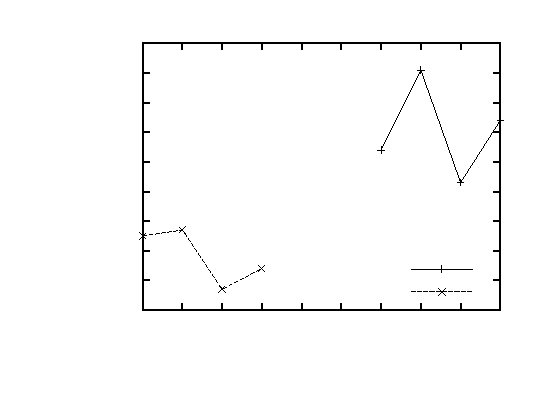
\includegraphics{tagged-sequential-plot}}%
    \gplfronttext
  \end{picture}%
\endgroup

		\caption{Speedup using the tagged sequential prefetcher.}
		\label{figure:ts}
	\end{centering}
\end{figure}

As it can be observed in Figure~\ref{figure:ts}, that the TS configuration with
the best overall benchmark score has degree 1 and distance 6. The speedup with
this configuration is 1.030. In general, degree 1 gives decent results, except
when the distance is 10. Increasing the degree only worsens performance.

The ``\emph{ammp}'' and ``\emph{twolf}'' benchmarks gave the lowest speedups,
with a speedup of 0.759 and 0.983 respectively (speedup results below 1.000
means the prefetcher actually slows down the application).

This is expected as those applications need to fetch instructions/data from
random locations~\cite[Sec.~4.2]{spec2000-memory}, making it very difficult for
the TS prefetcher to get any benefit from sequential fetching, which relies on
spatial locality.

\subsection{DCPT Results}

The figures below show the results from varying only one of the parameters while
keeping the others constant.

\begin{figure}[h!]
	\begin{centering}
		% GNUPLOT: LaTeX picture with Postscript
\begingroup
  \makeatletter
  \providecommand\color[2][]{%
    \GenericError{(gnuplot) \space\space\space\@spaces}{%
      Package color not loaded in conjunction with
      terminal option `colourtext'%
    }{See the gnuplot documentation for explanation.%
    }{Either use 'blacktext' in gnuplot or load the package
      color.sty in LaTeX.}%
    \renewcommand\color[2][]{}%
  }%
  \providecommand\includegraphics[2][]{%
    \GenericError{(gnuplot) \space\space\space\@spaces}{%
      Package graphicx or graphics not loaded%
    }{See the gnuplot documentation for explanation.%
    }{The gnuplot epslatex terminal needs graphicx.sty or graphics.sty.}%
    \renewcommand\includegraphics[2][]{}%
  }%
  \providecommand\rotatebox[2]{#2}%
  \@ifundefined{ifGPcolor}{%
    \newif\ifGPcolor
    \GPcolorfalse
  }{}%
  \@ifundefined{ifGPblacktext}{%
    \newif\ifGPblacktext
    \GPblacktexttrue
  }{}%
  % define a \g@addto@macro without @ in the name:
  \let\gplgaddtomacro\g@addto@macro
  % define empty templates for all commands taking text:
  \gdef\gplbacktext{}%
  \gdef\gplfronttext{}%
  \makeatother
  \ifGPblacktext
    % no textcolor at all
    \def\colorrgb#1{}%
    \def\colorgray#1{}%
  \else
    % gray or color?
    \ifGPcolor
      \def\colorrgb#1{\color[rgb]{#1}}%
      \def\colorgray#1{\color[gray]{#1}}%
      \expandafter\def\csname LTw\endcsname{\color{white}}%
      \expandafter\def\csname LTb\endcsname{\color{black}}%
      \expandafter\def\csname LTa\endcsname{\color{black}}%
      \expandafter\def\csname LT0\endcsname{\color[rgb]{1,0,0}}%
      \expandafter\def\csname LT1\endcsname{\color[rgb]{0,1,0}}%
      \expandafter\def\csname LT2\endcsname{\color[rgb]{0,0,1}}%
      \expandafter\def\csname LT3\endcsname{\color[rgb]{1,0,1}}%
      \expandafter\def\csname LT4\endcsname{\color[rgb]{0,1,1}}%
      \expandafter\def\csname LT5\endcsname{\color[rgb]{1,1,0}}%
      \expandafter\def\csname LT6\endcsname{\color[rgb]{0,0,0}}%
      \expandafter\def\csname LT7\endcsname{\color[rgb]{1,0.3,0}}%
      \expandafter\def\csname LT8\endcsname{\color[rgb]{0.5,0.5,0.5}}%
    \else
      % gray
      \def\colorrgb#1{\color{black}}%
      \def\colorgray#1{\color[gray]{#1}}%
      \expandafter\def\csname LTw\endcsname{\color{white}}%
      \expandafter\def\csname LTb\endcsname{\color{black}}%
      \expandafter\def\csname LTa\endcsname{\color{black}}%
      \expandafter\def\csname LT0\endcsname{\color{black}}%
      \expandafter\def\csname LT1\endcsname{\color{black}}%
      \expandafter\def\csname LT2\endcsname{\color{black}}%
      \expandafter\def\csname LT3\endcsname{\color{black}}%
      \expandafter\def\csname LT4\endcsname{\color{black}}%
      \expandafter\def\csname LT5\endcsname{\color{black}}%
      \expandafter\def\csname LT6\endcsname{\color{black}}%
      \expandafter\def\csname LT7\endcsname{\color{black}}%
      \expandafter\def\csname LT8\endcsname{\color{black}}%
    \fi
  \fi
  \setlength{\unitlength}{0.0500bp}%
  \begin{picture}(5040.00,3528.00)%
    \gplgaddtomacro\gplbacktext{%
      \csname LTb\endcsname%
      \put(1210,704){\makebox(0,0)[r]{\strut{} 1.016}}%
      \put(1210,988){\makebox(0,0)[r]{\strut{} 1.018}}%
      \put(1210,1273){\makebox(0,0)[r]{\strut{} 1.02}}%
      \put(1210,1557){\makebox(0,0)[r]{\strut{} 1.022}}%
      \put(1210,1841){\makebox(0,0)[r]{\strut{} 1.024}}%
      \put(1210,2126){\makebox(0,0)[r]{\strut{} 1.026}}%
      \put(1210,2410){\makebox(0,0)[r]{\strut{} 1.028}}%
      \put(1210,2694){\makebox(0,0)[r]{\strut{} 1.03}}%
      \put(1210,2979){\makebox(0,0)[r]{\strut{} 1.032}}%
      \put(1210,3263){\makebox(0,0)[r]{\strut{} 1.034}}%
      \put(1469,484){\makebox(0,0){\strut{}14}}%
      \put(1723,484){\makebox(0,0){\strut{}16}}%
      \put(1977,484){\makebox(0,0){\strut{}18}}%
      \put(2231,484){\makebox(0,0){\strut{}19}}%
      \put(2485,484){\makebox(0,0){\strut{}20}}%
      \put(2739,484){\makebox(0,0){\strut{}21}}%
      \put(2993,484){\makebox(0,0){\strut{}22}}%
      \put(3246,484){\makebox(0,0){\strut{}24}}%
      \put(3500,484){\makebox(0,0){\strut{}30}}%
      \put(3754,484){\makebox(0,0){\strut{}35}}%
      \put(4008,484){\makebox(0,0){\strut{}40}}%
      \put(4262,484){\makebox(0,0){\strut{}45}}%
      \put(4516,484){\makebox(0,0){\strut{}48}}%
      \put(176,1983){\rotatebox{-270}{\makebox(0,0){\strut{}Speedup}}}%
      \put(2992,154){\makebox(0,0){\strut{}Deltas per entry}}%
    }%
    \gplgaddtomacro\gplfronttext{%
    }%
    \gplbacktext
    \put(0,0){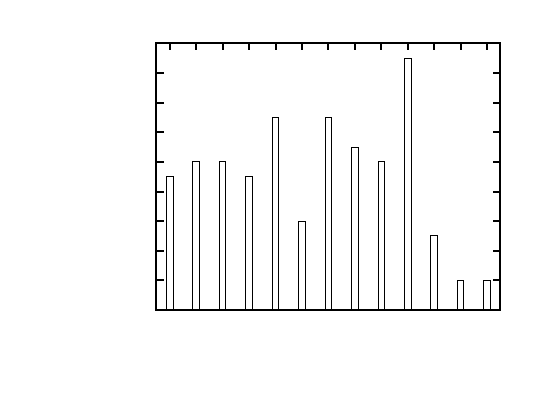
\includegraphics{DCPT-num-deltas-plot}}%
    \gplfronttext
  \end{picture}%
\endgroup

		\caption{Speedup using the DCPT prefetcher with 98 entries, and 12 bits for each delta.}
		\label{figure:dcpt-num-deltas}
	\end{centering}
\end{figure}

\begin{figure}[h!]
	\begin{centering}
		% GNUPLOT: LaTeX picture with Postscript
\begingroup
  \makeatletter
  \providecommand\color[2][]{%
    \GenericError{(gnuplot) \space\space\space\@spaces}{%
      Package color not loaded in conjunction with
      terminal option `colourtext'%
    }{See the gnuplot documentation for explanation.%
    }{Either use 'blacktext' in gnuplot or load the package
      color.sty in LaTeX.}%
    \renewcommand\color[2][]{}%
  }%
  \providecommand\includegraphics[2][]{%
    \GenericError{(gnuplot) \space\space\space\@spaces}{%
      Package graphicx or graphics not loaded%
    }{See the gnuplot documentation for explanation.%
    }{The gnuplot epslatex terminal needs graphicx.sty or graphics.sty.}%
    \renewcommand\includegraphics[2][]{}%
  }%
  \providecommand\rotatebox[2]{#2}%
  \@ifundefined{ifGPcolor}{%
    \newif\ifGPcolor
    \GPcolorfalse
  }{}%
  \@ifundefined{ifGPblacktext}{%
    \newif\ifGPblacktext
    \GPblacktexttrue
  }{}%
  % define a \g@addto@macro without @ in the name:
  \let\gplgaddtomacro\g@addto@macro
  % define empty templates for all commands taking text:
  \gdef\gplbacktext{}%
  \gdef\gplfronttext{}%
  \makeatother
  \ifGPblacktext
    % no textcolor at all
    \def\colorrgb#1{}%
    \def\colorgray#1{}%
  \else
    % gray or color?
    \ifGPcolor
      \def\colorrgb#1{\color[rgb]{#1}}%
      \def\colorgray#1{\color[gray]{#1}}%
      \expandafter\def\csname LTw\endcsname{\color{white}}%
      \expandafter\def\csname LTb\endcsname{\color{black}}%
      \expandafter\def\csname LTa\endcsname{\color{black}}%
      \expandafter\def\csname LT0\endcsname{\color[rgb]{1,0,0}}%
      \expandafter\def\csname LT1\endcsname{\color[rgb]{0,1,0}}%
      \expandafter\def\csname LT2\endcsname{\color[rgb]{0,0,1}}%
      \expandafter\def\csname LT3\endcsname{\color[rgb]{1,0,1}}%
      \expandafter\def\csname LT4\endcsname{\color[rgb]{0,1,1}}%
      \expandafter\def\csname LT5\endcsname{\color[rgb]{1,1,0}}%
      \expandafter\def\csname LT6\endcsname{\color[rgb]{0,0,0}}%
      \expandafter\def\csname LT7\endcsname{\color[rgb]{1,0.3,0}}%
      \expandafter\def\csname LT8\endcsname{\color[rgb]{0.5,0.5,0.5}}%
    \else
      % gray
      \def\colorrgb#1{\color{black}}%
      \def\colorgray#1{\color[gray]{#1}}%
      \expandafter\def\csname LTw\endcsname{\color{white}}%
      \expandafter\def\csname LTb\endcsname{\color{black}}%
      \expandafter\def\csname LTa\endcsname{\color{black}}%
      \expandafter\def\csname LT0\endcsname{\color{black}}%
      \expandafter\def\csname LT1\endcsname{\color{black}}%
      \expandafter\def\csname LT2\endcsname{\color{black}}%
      \expandafter\def\csname LT3\endcsname{\color{black}}%
      \expandafter\def\csname LT4\endcsname{\color{black}}%
      \expandafter\def\csname LT5\endcsname{\color{black}}%
      \expandafter\def\csname LT6\endcsname{\color{black}}%
      \expandafter\def\csname LT7\endcsname{\color{black}}%
      \expandafter\def\csname LT8\endcsname{\color{black}}%
    \fi
  \fi
  \setlength{\unitlength}{0.0500bp}%
  \begin{picture}(5040.00,3528.00)%
    \gplgaddtomacro\gplbacktext{%
      \csname LTb\endcsname%
      \put(1210,704){\makebox(0,0)[r]{\strut{} 1.017}}%
      \put(1210,988){\makebox(0,0)[r]{\strut{} 1.018}}%
      \put(1210,1273){\makebox(0,0)[r]{\strut{} 1.019}}%
      \put(1210,1557){\makebox(0,0)[r]{\strut{} 1.02}}%
      \put(1210,1841){\makebox(0,0)[r]{\strut{} 1.021}}%
      \put(1210,2126){\makebox(0,0)[r]{\strut{} 1.022}}%
      \put(1210,2410){\makebox(0,0)[r]{\strut{} 1.023}}%
      \put(1210,2694){\makebox(0,0)[r]{\strut{} 1.024}}%
      \put(1210,2979){\makebox(0,0)[r]{\strut{} 1.025}}%
      \put(1210,3263){\makebox(0,0)[r]{\strut{} 1.026}}%
      \put(1578,484){\makebox(0,0){\strut{}90}}%
      \put(2049,484){\makebox(0,0){\strut{}98}}%
      \put(2521,484){\makebox(0,0){\strut{}120}}%
      \put(2992,484){\makebox(0,0){\strut{}140}}%
      \put(3464,484){\makebox(0,0){\strut{}160}}%
      \put(3936,484){\makebox(0,0){\strut{}180}}%
      \put(4407,484){\makebox(0,0){\strut{}196}}%
      \put(176,1983){\rotatebox{-270}{\makebox(0,0){\strut{}Speedup}}}%
      \put(2992,154){\makebox(0,0){\strut{}Number of entries in the table}}%
    }%
    \gplgaddtomacro\gplfronttext{%
    }%
    \gplbacktext
    \put(0,0){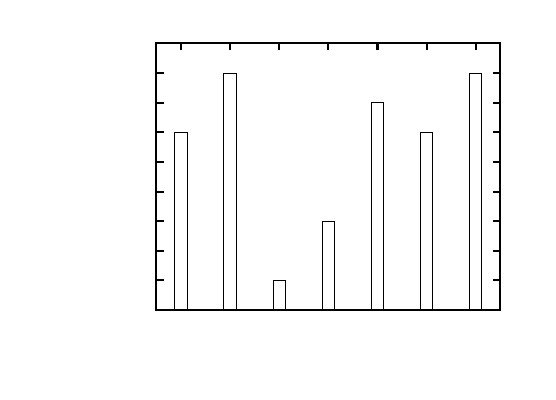
\includegraphics{DCPT-table-size-plot}}%
    \gplfronttext
  \end{picture}%
\endgroup

		\caption{Speedup using the DCPT prefetcher with 19 deltas per entry, and 12 bits for each delta.}
		\label{figure:dcpt-table-size}
	\end{centering}
\end{figure}

\begin{figure}[h!]
	\begin{centering}
		% GNUPLOT: LaTeX picture with Postscript
\begingroup
  \makeatletter
  \providecommand\color[2][]{%
    \GenericError{(gnuplot) \space\space\space\@spaces}{%
      Package color not loaded in conjunction with
      terminal option `colourtext'%
    }{See the gnuplot documentation for explanation.%
    }{Either use 'blacktext' in gnuplot or load the package
      color.sty in LaTeX.}%
    \renewcommand\color[2][]{}%
  }%
  \providecommand\includegraphics[2][]{%
    \GenericError{(gnuplot) \space\space\space\@spaces}{%
      Package graphicx or graphics not loaded%
    }{See the gnuplot documentation for explanation.%
    }{The gnuplot epslatex terminal needs graphicx.sty or graphics.sty.}%
    \renewcommand\includegraphics[2][]{}%
  }%
  \providecommand\rotatebox[2]{#2}%
  \@ifundefined{ifGPcolor}{%
    \newif\ifGPcolor
    \GPcolorfalse
  }{}%
  \@ifundefined{ifGPblacktext}{%
    \newif\ifGPblacktext
    \GPblacktexttrue
  }{}%
  % define a \g@addto@macro without @ in the name:
  \let\gplgaddtomacro\g@addto@macro
  % define empty templates for all commands taking text:
  \gdef\gplbacktext{}%
  \gdef\gplfronttext{}%
  \makeatother
  \ifGPblacktext
    % no textcolor at all
    \def\colorrgb#1{}%
    \def\colorgray#1{}%
  \else
    % gray or color?
    \ifGPcolor
      \def\colorrgb#1{\color[rgb]{#1}}%
      \def\colorgray#1{\color[gray]{#1}}%
      \expandafter\def\csname LTw\endcsname{\color{white}}%
      \expandafter\def\csname LTb\endcsname{\color{black}}%
      \expandafter\def\csname LTa\endcsname{\color{black}}%
      \expandafter\def\csname LT0\endcsname{\color[rgb]{1,0,0}}%
      \expandafter\def\csname LT1\endcsname{\color[rgb]{0,1,0}}%
      \expandafter\def\csname LT2\endcsname{\color[rgb]{0,0,1}}%
      \expandafter\def\csname LT3\endcsname{\color[rgb]{1,0,1}}%
      \expandafter\def\csname LT4\endcsname{\color[rgb]{0,1,1}}%
      \expandafter\def\csname LT5\endcsname{\color[rgb]{1,1,0}}%
      \expandafter\def\csname LT6\endcsname{\color[rgb]{0,0,0}}%
      \expandafter\def\csname LT7\endcsname{\color[rgb]{1,0.3,0}}%
      \expandafter\def\csname LT8\endcsname{\color[rgb]{0.5,0.5,0.5}}%
    \else
      % gray
      \def\colorrgb#1{\color{black}}%
      \def\colorgray#1{\color[gray]{#1}}%
      \expandafter\def\csname LTw\endcsname{\color{white}}%
      \expandafter\def\csname LTb\endcsname{\color{black}}%
      \expandafter\def\csname LTa\endcsname{\color{black}}%
      \expandafter\def\csname LT0\endcsname{\color{black}}%
      \expandafter\def\csname LT1\endcsname{\color{black}}%
      \expandafter\def\csname LT2\endcsname{\color{black}}%
      \expandafter\def\csname LT3\endcsname{\color{black}}%
      \expandafter\def\csname LT4\endcsname{\color{black}}%
      \expandafter\def\csname LT5\endcsname{\color{black}}%
      \expandafter\def\csname LT6\endcsname{\color{black}}%
      \expandafter\def\csname LT7\endcsname{\color{black}}%
      \expandafter\def\csname LT8\endcsname{\color{black}}%
    \fi
  \fi
  \setlength{\unitlength}{0.0500bp}%
  \begin{picture}(5040.00,3528.00)%
    \gplgaddtomacro\gplbacktext{%
      \csname LTb\endcsname%
      \put(1210,704){\makebox(0,0)[r]{\strut{} 0.995}}%
      \put(1210,1070){\makebox(0,0)[r]{\strut{} 1}}%
      \put(1210,1435){\makebox(0,0)[r]{\strut{} 1.005}}%
      \put(1210,1801){\makebox(0,0)[r]{\strut{} 1.01}}%
      \put(1210,2166){\makebox(0,0)[r]{\strut{} 1.015}}%
      \put(1210,2532){\makebox(0,0)[r]{\strut{} 1.02}}%
      \put(1210,2897){\makebox(0,0)[r]{\strut{} 1.025}}%
      \put(1210,3263){\makebox(0,0)[r]{\strut{} 1.03}}%
      \put(1617,484){\makebox(0,0){\strut{}7}}%
      \put(2167,484){\makebox(0,0){\strut{}11}}%
      \put(2717,484){\makebox(0,0){\strut{}12}}%
      \put(3268,484){\makebox(0,0){\strut{}13}}%
      \put(3818,484){\makebox(0,0){\strut{}17}}%
      \put(4368,484){\makebox(0,0){\strut{}28}}%
      \put(176,1983){\rotatebox{-270}{\makebox(0,0){\strut{}Speedup}}}%
      \put(2992,154){\makebox(0,0){\strut{}Bits per delta}}%
    }%
    \gplgaddtomacro\gplfronttext{%
    }%
    \gplbacktext
    \put(0,0){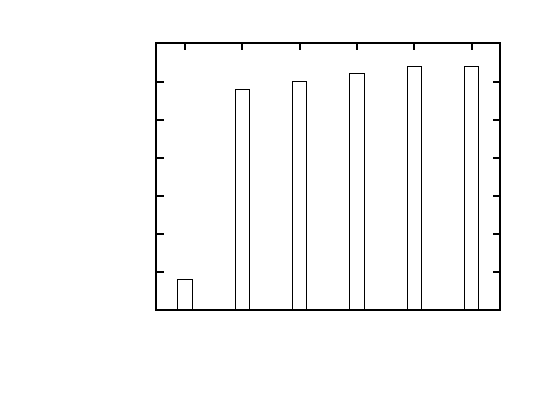
\includegraphics{DCPT-delta-bits-plot}}%
    \gplfronttext
  \end{picture}%
\endgroup

		\caption{Speedup using the DCPT prefetcher with 98 entries, and 19 deltas per entry.}
		\label{figure:dcpt-delta-bits}
	\end{centering}
\end{figure}

We obtain the best results with 98 or 196 entries in the table. In order to save
size, further simulations are therefore done with 98 entries. The simulations
above clearly shows that the optimal number of deltas per entry is 35. The
number of bits per delta needs to be at least 11, but the performance is best
with 17 or more bits per delta.

For further optimization, we combine the parameter values that give the best
preformance and additionally test them with some minor variations. The results
of this is shown in tables~\ref{tab:numdelta},~\ref{tab:tablesize},
and~\ref{tab:deltabits}.

\begin{table}[h!]
	\centering
	\begin{tabular}{|l|l|l|l|l|l|l|}
		\hline
		32	& 33	& 34	& \textbf{35}	& 36	& 37	& 38	\\
		\hline
		1.028 & 1.029 & 1.029 & \textbf{1.033} & 1.027 & 1.028 & 1.027 \\
		\hline
	\end{tabular}
	\smallskip
	\caption{Speedup for number of deltas around the best configuration}
	\label{tab:numdelta}
\end{table}

\begin{table}[h!]
	\centering
	\begin{tabular}{|l|l|l|l|l|l|l|}
		\hline
		95	& 96	& 97	& \textbf{98}	& 99	& 100	& 101	\\
		\hline
		1.020 & 1.017 & 1.025 & \textbf{1.033} & 1.026 & 1.015 & 1.021 \\
		\hline
	\end{tabular}
	\smallskip
	\caption{Speedup with different number of entries around the best configuration}
	\label{tab:tablesize}
\end{table}

\begin{table}[h!]
	\centering
	\begin{tabular}{|l|l|l|l|l|}
		\hline
		\textbf{12}	& 13	& 14	& 15	& 16	\\
		\hline
		\textbf{1.033} & 1.026 & 1.028 & 1.029 & 1.028 \\
		\hline
	\end{tabular}
	\smallskip
	\caption{Speedup with different number of bits representing each delta around the best configuration}
	\label{tab:deltabits}
\end{table}

None of the variations proved better than the original one.

\subsection{Best Results}

Figure \ref{figure:benchmarks-plot} shows the results from each of the SPEC
CPU2000 benchmarks for both TS and DCPT with optmial parameter values.

\begin{figure}[h!]
	\begin{centering}
		\input{benchmarks-plot}
		\caption{Speedup on the individual benchmarks for the TS and DCPT configurations with highest average speedup.}
		\label{figure:benchmarks-plot}
	\end{centering}
\end{figure}

\todo[inline]{
- Prefetching: Best case is that all L2 accesses are hits\\
Sensitivity analysis: \\
- Check the impact of model assumptions on your
scheme}


\section{Discussion}

The results from the TS prefetcher shows that smaller degrees tend
to do better. Therefore we tried to do something similar with the DCPT by limiting the
number of prefetches generated by a single access, but the simulation
results show that this does not yield any improvements.


\section{Conclusion}
The conclusion goes here. 


\appendices
%\section{Proof of the First Zonklar Equation}
%Appendix one text goes here.

% you can choose not to have a title for an appendix
% if you want by leaving the argument blank
%\section{}
%Appendix two text goes here.

%\ifCLASSOPTIONcaptionsoff
%  \newpage
%\fi

\begin{thebibliography}{1}

\bibitem{grannaes}
M.~Grannaes, \emph{Reducing Memory Latency by
Improving Resource Utilization}, \hskip 1em plus
  0.5em minus 0.4em\relax Trondheim, Norway: NTNU, 2010.

\bibitem{user_doc}
\emph{TDT4260 Computer Architecture: 
M5 simulator system - User documentation}, \hskip 1em plus
  0.5em minus 0.4em\relax Trondheim, Norway: NTNU, 2014.
  
\bibitem{guidelines}
N.~Reissmann, \emph{TDT4260 Computer Architecture: 
Mini-Project Guidelines}, \hskip 1em plus
  0.5em minus 0.4em\relax Trondheim, Norway: NTNU, 2014.

\bibitem{dcpt}
M.~Grannaes et al., \emph{Storage Efficient Hardware 
Prefetching using Delta-Correlating Prediction Tables}, 
\hskip 1em plus
  0.5em minus 0.4em\relax Trondheim, Norway: NTNU, 2011.

\end{thebibliography}
\end{document}